\section{Weak Subjectivity Period}

To minimize the social consensus overhead, we want to identify the minimum cycle to update weak subjectivity checkpoints, called weak subjectivity periods.  The weak subjectivity period must be smaller than the minimum  time it takes for the condition of the long-range attacks to be established.  Specifically, it must be smaller than each of the following:
\begin{itemize}
\item $\E_1$:
The minimum number of epochs for $2/3$ of all active validators to exit.
\item $\E_2$:
The minimum number of epochs for the original validator set to diverge into two sets so that the (accountable) safety tolerance falls below a certain threshold, $\frac{1}{3} - D$. (We call $D$ safety decay.)
%where the size of their intersection falls below a certain threshold.
\end{itemize}

The computation of $\E_2$ is not straightforward, especially when the balance of validators changes over epochs.
For simplicity of presentation, we first analyze the weak subjectivity period in a simpler setting where all validators' balance are fixed to the same constant.
Later we analyze the effect of balance top-ups separately.

\subsection{Weak Subjectivity for Dynamic Validator Set with Unit Balance}

In this section, we analyze the weak subjectivity period in a simpler setting where the validator set changes over epochs but their balance is equally fixed to the same amount.

\begin{theorem}\label{thm:weak-subjectivity-unit-balance}
Let $N$ be the current total number of active validators.
Let $\delta$ be the validator activation and exit limit per epoch.\footnote{In the current configuration, $\delta$ is $\texttt{MIN\_PER\_EPOCH\_CHURN\_LIMIT} = 4$ when $N \le 2^{18}$, and $\floor{N \cdot \texttt{CHURN\_LIMIT\_QUOTIENT}^{-1}} = \floor{N \cdot 2^{-16}}$ otherwise.}
Let $D$ be the safety decay.
%where the accountable safety tolerance is $\frac{1}{3} - D$.
Then, given $0 \le D \le \frac{1}{3}$, the current weak subjectivity period must be smaller than $\frac{1}{2} DN /\delta$.
\end{theorem}
\begin{proof}
Recall that the weak subjectivity period must be smaller than $\min(\E_1,\E_2)$, where we claim that:
\[
\E_1 = \ceil{\frac{2N}{3\delta}}
\qquad\mathrm{and}\qquad
\E_2 = \ceil{\frac{DN}{2\delta}}
\]
The conclusion immediately follows the above claim since $0 \le D \le \frac{1}{3}$.
Now let us prove the above claim.

Let us first prove the claim for $\E_1$.
By Lemma~\ref{lem:best-strategy}, the maximum number of (originally existing) validators that can exit over the next $n$ epochs is $\delta n$.
%where $\delta$ is fixed to a constant when the total number of validators $N$ is small, and is proportional to $N$ otherwise.\footnote{In the current configuration, $\delta$ is $\texttt{MIN\_PER\_EPOCH\_CHURN\_LIMIT} = 4$ when $N \le 2^{18}$, and $\floor{N \cdot \texttt{CHURN\_LIMIT\_QUOTIENT}^{-1}} = \floor{N \cdot 2^{-16}}$ otherwise.}
Thus, the minimum number of epochs for $\frac{2}{3} N$ validators to exit, $\E_1$, is $\ceil{\frac{2}{3}N/\delta}$.

Now let us prove the claim for $\E_2$.
Let $V_0$ be the current set of all validators, that is, $|V_0| = N$.
Suppose that $V_0$ diverges into two sets $V_L$ and $V_R$ over two chains at a later epoch.
Then, by Lemma~\ref{lem:safety-tolerance}, the number of slashable validators $\ST(V_L,V_R)$ is $\max(0, |V_L \cap V_R| - \frac{1}{3} (|V_L| + |V_R|))$, which can be rewritten as:
\[
\ST(V_L,V_R) = \frac{1}{3} \max(0, |V_L \cap V_R| - |V_L-V_R| - |V_R-V_L|)
\]
Now we need to calculate the minimum number of epochs required for:
\begin{equation}\label{eq:st-le-d}
\frac{\ST(V_L,V_R)}{N} \le \frac{1}{3} - D
\end{equation}
This boils down to finding the best strategy to minimize $\ST(V_L,V_R)$ as quickly as possible.
Note that $\ST(V_L,V_R)$ is minimized when $V_L \cap V_R$ is minimized and both $|V_L-V_R|$ and $|V_R-V_L|$ is maximized.
That can be achieved by activating different new validators in different chains as much as possible, and removing different originally existing validators in different chains as much as possible.
Thus, by Lemma~\ref{lem:best-strategy}, the best strategy to minimize $\ST(V_L,V_R)$ as quickly as possible is that:
\begin{itemize}
\item Activate new validators at the maximum activation limit per epoch, where the newly activated validators of the two chains have to be disjoint, and
\item Remove originally existing validators at the maximum exit limit per epoch, where the exited validators of the two chains have to be disjoint.
\end{itemize}
Let $A_L$ and $A_R$ be the set of new validators activated in each of the two chains, respectively, during the next $n$ epochs following the above strategy.
Similarly, let $E_L$ and $E_R$ be the set of existing validators removed in each of the two chains, respectively.
By Lemma~\ref{lem:best-strategy}, we have $A_L = A_R = E_L = E_R = \delta n$.
%Figure~\ref{fig:after-n-epoch} 
The following diagram illustrates how $V_0$ diverges to $V_L$ and $V_R$ over the $n$ epochs following the best strategy, where $V_0$ is denoted by the blue area ($V_0 = (V_L \cap V_R) + E_L + E_R$), $V_L$ is the partial rectangle in the left ($V_L = V + A_L - E_L$), and $V_R$ is the partial rectangle in the right ($V_R = V + A_R - E_R$).
\begin{center}
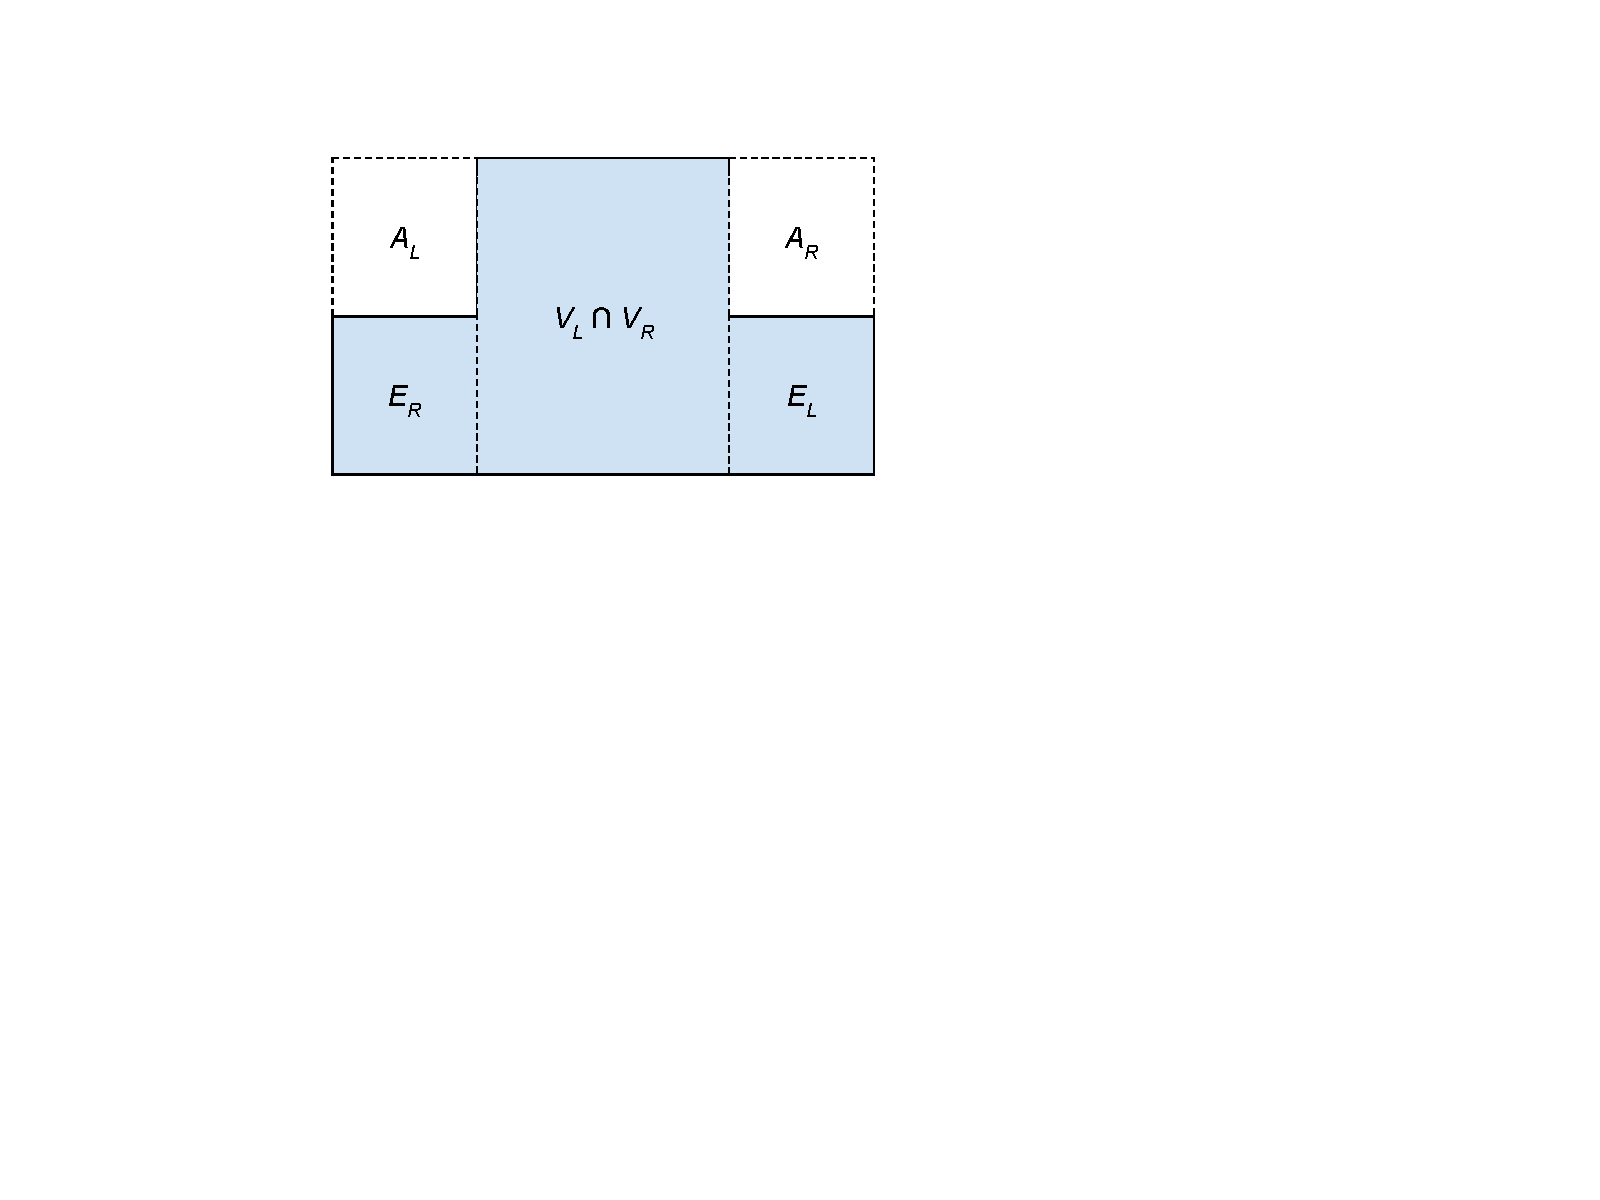
\includegraphics[width=.5\columnwidth]{after-n-epoch.pdf}
\end{center}
Now we have $\ST(V_L,V_R)$ after the next $n$ epochs following the best strategy as follows:
\begin{align*}
\ST(V_L,V_R) & = \frac{1}{3} \max(0, |V_L \cap V_R| - |V_L-V_R| - |V_R-V_L|) \\
& = \frac{1}{3} \max(0, (|V_0| - E_L - E_R) - (A_L+E_R) - (A_R+E_L)) \\
& = \frac{1}{3}\max(0, |V_0| - 6\delta n)
\end{align*}
Thus, given the safety decay $0 \le D \le \frac{1}{3}$, the minimum number of epochs for \eqref{eq:st-le-d}, $\E_2$, is $\ceil{\frac{1}{2}DN/\delta}$.
\qed
\end{proof}

%\begin{figure}[t]
%\centering
%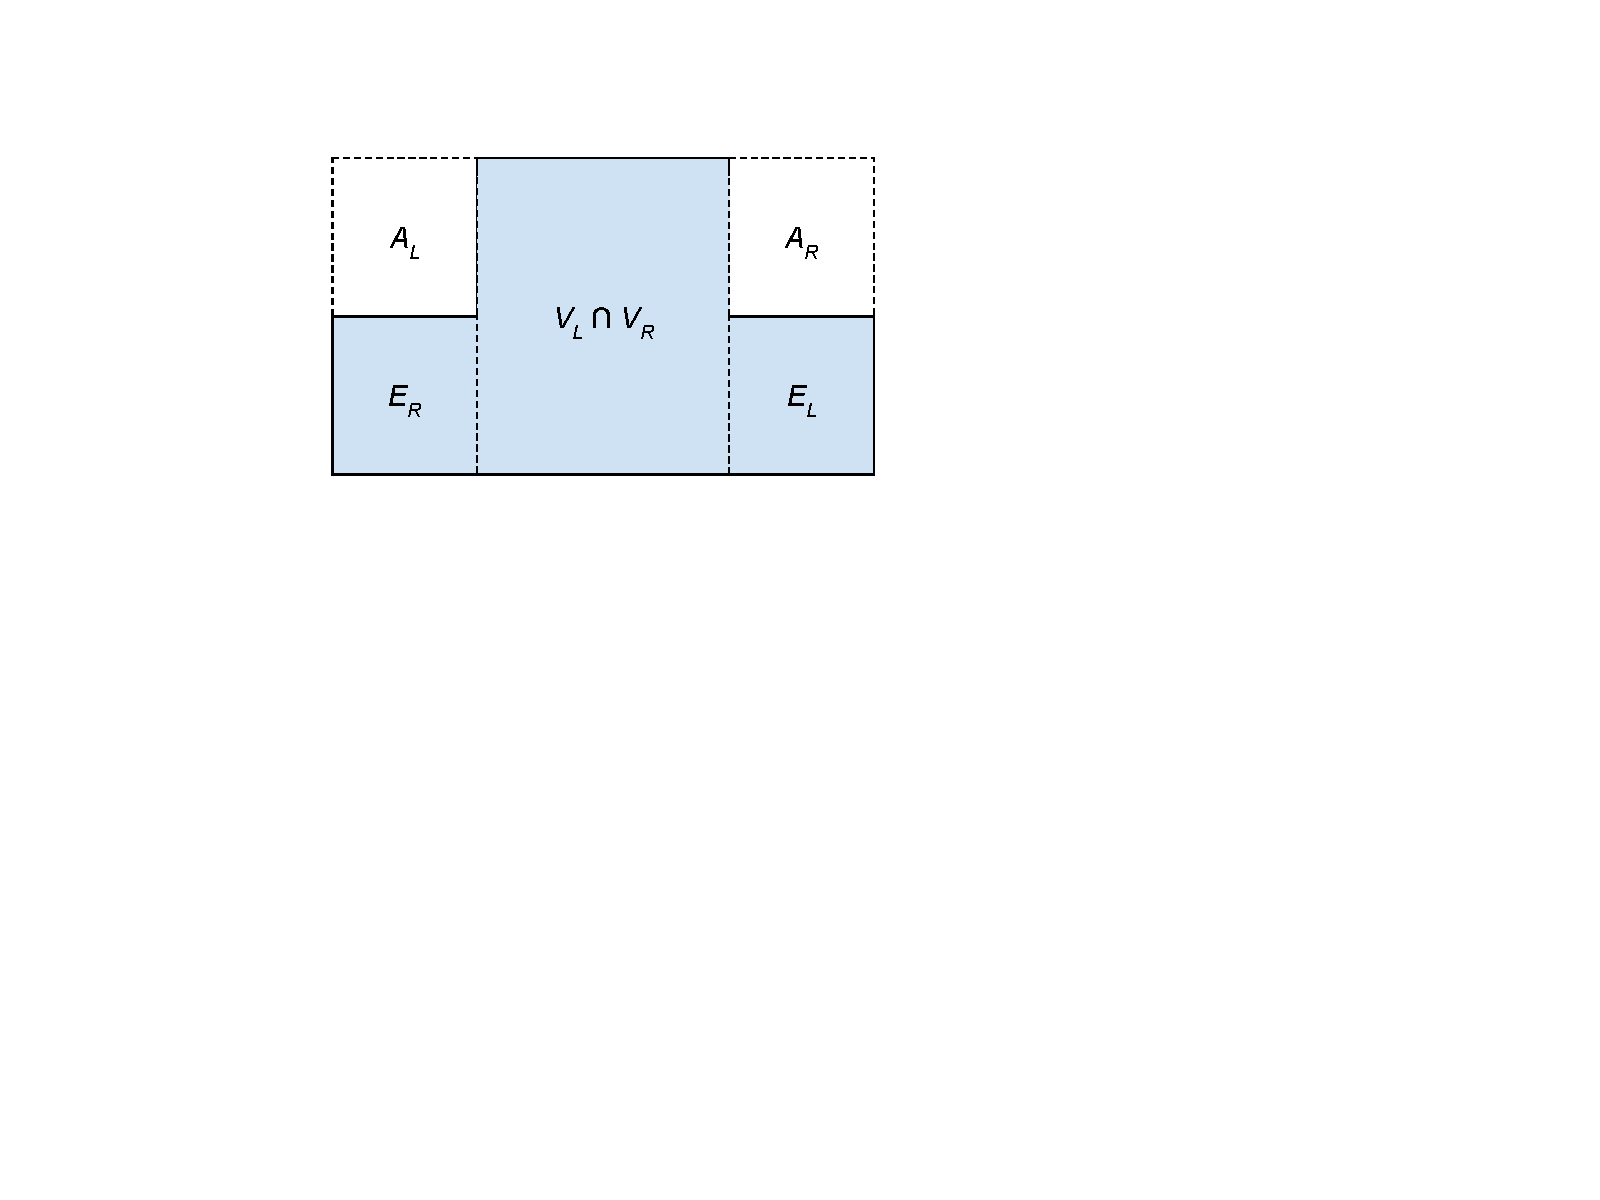
\includegraphics[width=.5\columnwidth]{after-n-epoch.pdf}
%\caption{Illustration of $V_0$ diverging to $V_L$ and $V_R$ over different chains, where $V_0 = (V_L \cap V_R) + E_L + E_R$, $V_L = V_0 + A_L - E_L$, and $V_R = V_0 + A_R - E_R$.}
%\label{fig:after-n-epoch}
%\end{figure}

\begin{lemma}[Maximum Validator Exits]\label{lem:best-strategy}
Let $N$ be the current total number of active validators.
Let $\delta(x)$ be the validator activation and exit limit per epoch for the given set of all active validators whose size is $x$.
Suppose that $\delta(x)$ is proportional to $x$ with a fixed lower bound, that is, that there exist constants $\delta_0$, $x_0$, and $\rho < 1$, such that $\delta(x) = \max(\delta_0, \floor{\rho x})$ where $\delta_0 = \rho x_0$.
Also suppose that $\rho$ is sufficiently small compared to $\delta_0$, that is, $\rho\delta_0 < 1$.
%
Then, the maximum number of validators that can exit over the next $n$ epochs is $n\delta(N)$.
\end{lemma}
\begin{proof}
First let us show that there exists a strategy that can remove $n\delta(N)$ validators over $n$ epochs.
The strategy is simply to remove validators at the maximum exit limit while activating new validators at the maximum activation limit.
Since the maximum activation limit is equal to the maximum exit limit, the total number of validators does not change over the $n$ epochs under the strategy, thus $\delta(N)$ validators can exit for every epoch over the $n$ epochs.

Now, let us show that the simple strategy is optimal.
Let us first consider the case of $N \ge k_0$, that is, $\delta(N) = \rho N$.
Assume that there is a strategy $S$ that can remove more validators than the simple strategy.
Then, first, it is clear that the strategy $S$ has to activate new validators at the max per-epoch limit to maximize the size of the validator set, which in turn maximizes the max exit limit.
Now, assume that the strategy $S$ removes existing validators at the maximum rate \emph{only} after the first $k$ epochs.\footnote{Note that the strategy $S$ is better than any other strategy that removes validators at the maximum rate only for some $(n-k)$ epochs rather than the last $(n-k)$ epochs.  That is because the total number of validators at each of those epochs is not greater than that of the last epochs.  Similarly, the strategy $S$ is better than any strategy that removes fewer validators than the exit limit but over multiple epochs.  For example, removing validators up to only 50\% of the exit limit over two epochs is worse than removing validators at the max rate at only the last epoch, because the exit limit for the latter is higher than that of the former.}
Then, after the first $k$ epochs, the total number of active validators becomes $N' = N(1+\rho)^k$, and thus the total number of removed validators is $N'\rho(n-k)$, that is, $N(1+\rho)^k\rho(n-k)$.
However, we have:\footnote{Graphically, \url{https://www.desmos.com/calculator/ooq6jzbpzb}}
\begin{equation}\label{eq:optimal}
N(1+\rho)^k\rho(n-k) \le N\rho n \quad \textrm{ for } 0 \le k \le n \le \rho^{-1} \textrm{ and } 0 \le \rho < 1
\end{equation}
where the equality holds only when $k = 0$.
This means that the strategy $S$ is not better than the simple strategy, which is a contradiction, thus we conclude that the simple strategy is optimal.
Note that we consider only $n \le \rho^{-1}$, since all of the originally existing validators are able to completely exit over the $\rho^{-1}$ epochs in the simple strategy.

Similarly in case of $N < k_0$, it is optimal to keep removing validators at the max limit from the first epoch, because the max exit limit is fixed to the constant $\delta_0$ while $N$ is sufficiently small such that $N + \delta_0 \le k_0$.
Even in the case of $N + \delta_0 > k_0$, we have $\delta(N + \delta_0) = \delta_0$ because $\rho\delta_0 < 1$.
Note that once the total validator set size becomes greater than $k_0$, it follows the above reasoning.
\qed
\end{proof}

\begin{remark}
Let us give an approximate (but intuitive) analysis of \eqref{eq:optimal}.
When $0 \le \rho \ll 1$, (which is the case in the current configuration for a large $N$), $(1+\rho)^k$ can be approximated to $(1+k\rho)$.
Thus,
$N(1+\rho)^k\rho(n-k) - N\rho n$
can be approximated to:
$N(1+k\rho)\rho(n-k) - N\rho n$,
which can be simplified to:
$N\rho k(-\rho k+\rho n-1)$,
whose maximum is 0 at $k = 0$ (for $0 \le k \le n \le \rho^{-1}$ and $0 \le \rho \ll 1$), since it is a $\cap$-shaped parabola (opens downward) with the roots 0 and $n - \rho^{-1} \le 0$.
\end{remark}

\begin{remark}
There could exist a better strategy if the activation limit is bigger than the exit limit.  For simplicity, suppose that the activation limit is bigger than the exit limit for the first $k$ epochs in the strategy $S$.  Then, the number of removed validators under the strategy $S$ is $N(1+a)^ke(n-k)$, where $a$ is the activation limit, and $e$ is the exit limit, while that of the simple strategy is $Nen$.  Then there exists a non-zero $k$ such that $N(1+a)^ke(n-k) > Nen$.\footnote{Graphically, \url{https://www.desmos.com/calculator/1vmjuxciiy}}  This means that it could be better to add new validators without removing any existing ones for a while to quickly increase the total number of validators, and then remove validators later at a much higher exit rate.  However, such a strategy does not outperform the simple strategy when the activation limit is not greater than the exit limit.
\end{remark}

Below we analyze the number of slashable validators in case that conflicting blocks are justified (and later finalized) under two different validator sets (on two different chains) at the same epoch.

\begin{lemma}[Minimum Slashable Validators]\label{lem:safety-tolerance}
Let $X$ and $Y$ be the two different validator sets on two different chains at the same epoch.
Then, for the given $X$ and $Y$, the minimum number of validators\footnote{Here we assume the unit stake balance model for simplicity.} who must have violated the slashing conditions in order for two conflicting blocks to be justified, written as $\ST(X,Y)$, is given as follows:\footnote{Note that in the ideal case of $X = Y$, we have $\ST(X,Y) = \frac{1}{3} \cdot |X|$, which agrees on the ideal safety tolerance.}
\[
\ST(X,Y) = \max(0, |X \cap Y| - \frac{|X| + |Y|}{3})
\]
\end{lemma}
\begin{proof}
To justify (and later finalize) conflicting blocks, say $A$ and $B$, we need votes from 2/3 of both $X$ and $Y$, say 2/3 of $X$ voting for $A$, and 2/3 of $Y$ voting for $B$.  Now the question is what is the minimum number of validators (who belong to both $X$ and $Y$) who must have voted for both $A$ and $B$.  To minimize the number of double-voted validators, all the validators in $X-Y$ and $Y-X$ must vote for $A$ and $B$, respectively.

Here we have two cases.  If either $|X-Y|$ or $|Y-X|$ is greater than or equal to 2/3 of $X$ and $Y$, respectively, then no one needs to double-vote, that is, the safety tolerance is zero, which agrees on the above formula.

So, now let us assume that both $|X-Y|$ and $|Y-X|$ is smaller than 2/3 of $X$ and $Y$, respectively.  Then, there should exist some validators in $X \cap Y$ who voted for $A$, and there should also exist some (possibly different) validators in $X \cap Y$ who voted for $B$.  Here, the (minimum) size of the former and the latter must be $\frac{2}{3} |X| - |X-Y|$, and $\frac{2}{3} |Y| - |Y-X|$, respectively.  Then, by the pigeonhole principle, the following number of validators must have double-voted:
\begin{align*}
& \max(0, (\frac{2}{3} |X| - |X-Y|) + (\frac{2}{3} |Y| - |Y-X|) - |X \cap Y|) \\
= & \max(0, (\frac{2}{3} |X| - (|X| - |X \cap Y|)) + (\frac{2}{3} |Y| - (|Y| - |X \cap Y|)) - |X \cap Y|) \\
= & \max(0, |X \cap Y| - \frac{1}{3} (|X| + |Y|))
\end{align*}
\qed
\end{proof}

\subsection{Weak Subjectivity for Static Validator Set with Balance Top-ups}

Validators whose balance falls below a certain threshold (16 ETH in the current configuration) are subject to removal, and they are allowed to top up their balance to avoid that.  Since the balance top-up essentially has a similar effect to adding new validators, it affects the weak subjectivity period.

In this section, we analyze the effect of balance top-ups on the weak subjectivity period.
To highlight its sole effect, here we assume the static validator set, where no additions or removals of validators are allowed.

\begin{lemma}[Potential Minimum Safety Tolerance]\label{lem:potential-safety-tolerance}
Assume the static validator set.
Let $N$ be the total number of validators.
Let $T$ be the maximum effective balance per validator.
Let $t$ be the average effective balance of all active validators at a certain point, that is, the total effective balance at that point is $tN$.
Let $\Delta$ be the number of validators allowed to top-up their balance per epoch.\footnote{In the current configuration, $\Delta = \texttt{MAX\_DEPOSITS} \times \texttt{SLOTS\_PER\_EPOCH} = 512$.}
%
Then, there exists an adversarial scenario where after a certain number of epochs, the (accountable) safety tolerance can be reduced to the following:\footnote{In the ideal case of $t = T$, this agrees on the ideal safety tolerance 1/3.}
\begin{equation}\label{eq:minimum-safety-tolerance}
\frac{2t - T}{4t - T} \quad (\text{for } \frac{T}{2} \le t \le T)
\end{equation}
The number of epochs required for \eqref{eq:minimum-safety-tolerance} can be as small as:
\begin{equation}\label{eq:min-epochs}
\frac{tN}{\Delta (4t - T)} \quad (\text{for } \frac{T}{2} \le t < T)
\end{equation}
%
%In case that there is no other way to update the balance of validators than the balance top-ups, \eqref{eq:minimum-safety-tolerance} is the lower bound, and \eqref{eq:min-epochs} is the minimum.
\end{lemma}
\begin{proof}
Let us present such an adversarial scenario.
Suppose that the validator set is split into the following three subsets, where $P$ and $Q$ denote the size of the corresponding subset, that is, $N = P + Q + P$.  For simplicity, we assume that the average balance of every subset is $t$.
\begin{center}
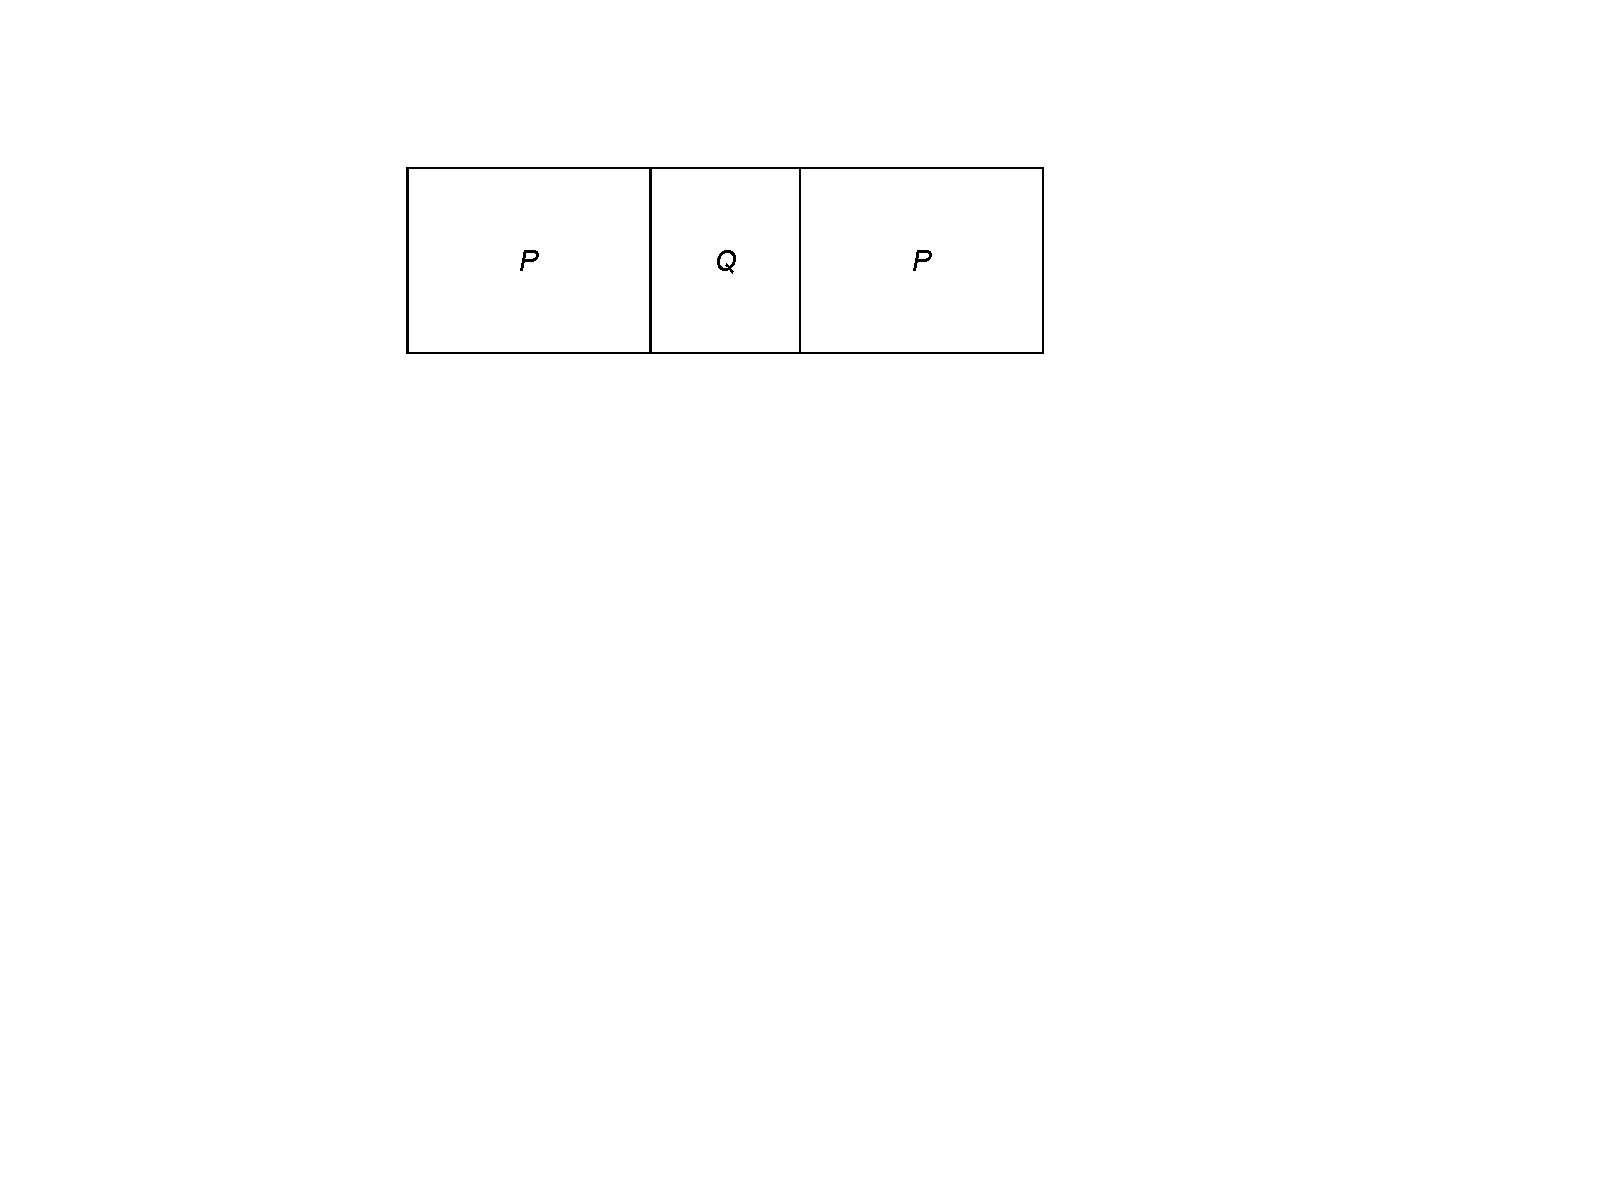
\includegraphics[width=.5\columnwidth]{balance-top-ups.pdf}
\end{center}
Now, suppose that two chains $X$ and $Y$ are created starting from this, where on chain $X$ (and $Y$), the $P$ validators in the left (and the right, respectively) top-up their balance to the (effective) maximum $T$.  Then suppose that the left $P$ validators in chain $X$ vote for a block $A$, the right $P$ in chain $Y$ vote for a conflicting block $B$, and the $Q$ validators in the middle double-vote for both $A$ and $B$.

Now, let us calculate the minimum $Q$ required for the conflicting blocks $A$ and $B$ to be justified (and later finalized).  First, we have that the total amount of stake in chain $X$ or $Y$ is $TP + tQ + tP$, and the weight of votes for block $A$ or $B$ is $TP + tQ$.  Then, $TP + tQ$ must be at least $\frac{2}{3} (TP + tQ + tP)$ to justify block $A$ or $B$.  Since $N = 2P+Q$, the minimum $Q$ is $N(2t - T) / (4t - T)$, and the maximum $P$ is $tN / (4t - T)$.
Thus we can conclude since the safety tolerance is the minimum $Q / N$, and
the number of epochs required to top-up the balance of $P$ validators is $P/\Delta$.
\qed
\end{proof}

\begin{remark}
The minimum of \eqref{eq:minimum-safety-tolerance} is 0 at $t = T/2$, and its maximum is $N/3$ at $t = T$.  In other words, when the average balance of validators is a half of $T$ (which is 16 ETH in the current configuration), the safety tolerance can be reduced to 0, meaning that conflicting blocks can be finalized without any validators needing to violate the slashing conditions.  In the ideal case that the balance of every validator is $T$, \eqref{eq:minimum-safety-tolerance} agrees on the ideal safety tolerance 1/3.  Moreover, notably, when $t = \frac{3}{4} T$ (which is 24 ETH in the current configuration), the safety tolerance can be reduced to $\frac{1}{4}$ (i.e., $\sim$8\% safety decay).
\end{remark}

\subsection{Weak Subjectivity for Dynamic Validator Set with Balance Top-ups}

In this section, we put together the results of the previous sections, analyzing the weak subjectivity period for the dynamic validator set with allowing validators to top-up their balance.

\begin{theorem}[Weak Subjectivity Period]\label{thm:weak-subjectivity-balance-top-ups}
Let $N$ be the total number of validators.
Let $T$ be the maximum effective balance per validator.
Let $t$ be the average effective balance.
Let $\Delta$ be the per-epoch limit of balance top-ups.
Let $\delta$ be the per-epoch limit of validator activations and exits.
Let $D$ be the safety decay.
%
Assume that $\Delta \gg \delta$.
Then, given $0 \le D \le \frac{1}{3}$, and $\frac{T}{2} \le t \le T$, the current weak subjectivity period must be smaller than:\footnotemark
\begin{itemize}
\item Case $(\frac{1}{3} - D) < (2t - T)/(4t - T)$:
\[
\max\left(
\frac{N}{\delta} \cdot \frac{(\frac{1}{3} + 2D)t - (\frac{1}{3} + \frac{D}{2})T}{2t+T},~~
\frac{N}{\Delta} \cdot (\frac{1}{3} + \frac{D}{2}) % \frac{(\frac{2}{3} + D)t + (\frac{1}{3} + \frac{D}{2})T}{2t+T}
\right)
\]
\item Case $(\frac{1}{3} - D) \ge (2t - T)/(4t - T)$:
\[
\frac{3N}{2\Delta} \cdot \frac{tD}{T-t}
\]
\end{itemize}
\end{theorem}
\footnotetext{Note that the two cases agree on when $(\frac{1}{3} - D) = (2t - T)/(4t - T)$.
Specifically, the first argument of max() becomes 0, i.e., $(\frac{1}{3} + 2D)t - (\frac{1}{3} + \frac{D}{2})T = 0$,
and the second argument of max() becomes equal to the second case, i.e., $\frac{1}{3} + \frac{D}{2} = \frac{3}{2} \cdot \frac{tD}{T-t}$.}
\begin{proof}
Let us present an adversarial scenario of exploiting diverging validator sets.

\paragraph{Case 1:}

Let us first consider the case of $\frac{1}{3} - D < (2t - T)/(4t - T)$ for the given $D$ and $t$.
By Lemma~\ref{lem:potential-safety-tolerance}, the given safety decay cannot be achieved by the sole effect of balance top-ups.
Thus both validator activations/exits and balance top-ups are needed to obtain sufficiently diverging validator sets.
Suppose that the original validator set evolves over a certain number of epochs as in the following diagram, where $A_L$ and $A_R$ denote the number of newly activated validators on each of two chains respectively, $E_L$ and $E_R$ denote the number of removed validators on each of two chains respectively, and $P_L$ (as well as $E_R$) and $P_R$ (as well as $E_L$) denote the number of validators who topped up their balance to $T$ on each of two chains respectively during the period.
Also suppose that the two diverging validator sets evolve following the strategies presented in (the proof of) Theorem~\ref{thm:weak-subjectivity-unit-balance} and Lemma~\ref{lem:potential-safety-tolerance}.
Thus we have:
\begin{equation}\label{eq:a=e}
A_L = A_R = E_L = E_R \quad \text{and} \quad P_L = P_R
\end{equation}
and we omit the subscript when not needed.
The original validator set is denoted by the gray area, that is, $N = E_R + P_L + Q + P_R + E_L$.
For simplicity, we assume that the original average balance of each subset of validators (i.e., each of $E_*$, $P_*$, and $Q$) is uniformly $t$.
At this point, the total amount of stake for each of the two chains $\T = AT + ET + PT + Qt + Pt$, while the original total amount of stake $\T_0 = Nt = (2E + 2P + Q)t$.
\begin{center}
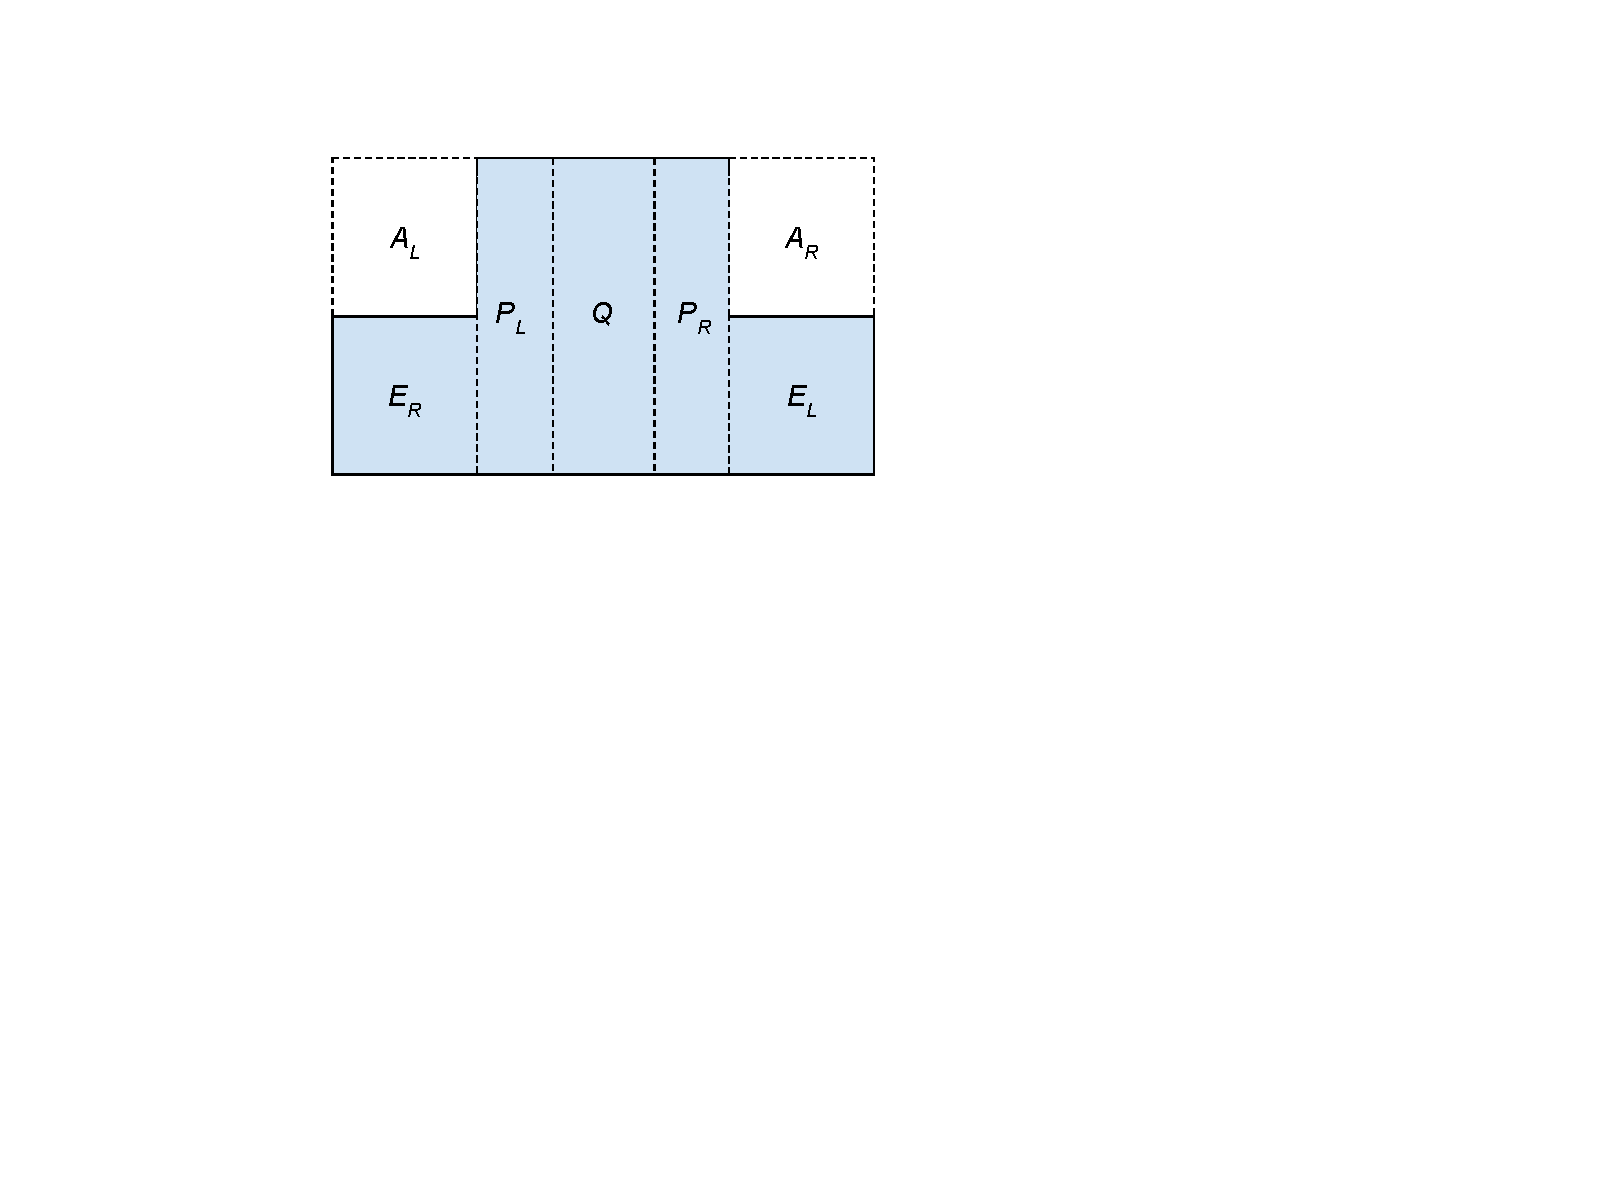
\includegraphics[width=.5\columnwidth]{after-n-epoch-balance-top-ups.pdf}
\end{center}
Now, suppose that the validators denoted by $A_L$, $E_R$, $P_L$, and $Q$ vote for a block on one of the two chains, and the validators denoted by $A_R$, $E_L$, $P_R$, and $Q$ vote for another block on the other chain at the same epoch.
Note that the $Q$ validators double-vote for both of the conflicting blocks.
To achieve the safety decay $D$, we need to have:
\begin{equation}\label{eq:q=dN}
Qt = (\frac{1}{3} - D) \cdot \T_0
\end{equation}
Also, to justify (and later finalize) each of the conflicting blocks, we need to have:
\begin{equation}\label{eq:a-e-p-q=s}
AT + ET + PT + Qt = \frac{2}{3} \T
\end{equation}
Now, by \eqref{eq:a=e}, \eqref{eq:q=dN}, and \eqref{eq:a-e-p-q=s}, we have:
\begin{align*}
E & = N \frac{(\frac{1}{3} + 2D)t - (\frac{1}{3} + \frac{D}{2})T}{2t+T} \\
P & = N \frac{(\frac{1}{3} - D)t + (\frac{2}{3} + D)T}{2t+T}
\end{align*}
and the number of epochs required for that is $\max(\frac{E}{\delta}, \frac{P+E}{\Delta})$.

\paragraph{Case 2:}

Now let us consider the remaining case of $\frac{1}{3} - D \ge (2t - T)/(4t - T)$.
By Lemma~\ref{lem:potential-safety-tolerance}, the given safety decay can be achieved by the sole effect of balance top-ups.
Moreover, $\Delta \gg \delta$, it takes a smaller number of epochs to rely only on the balance top-ups.
In this case, we have no validator activations or exits, i.e., $A = E = 0$, and only a subset of $P$ validators top-up their balance, i.e., there exist $P_1$ and $P_2$ such that $P = P_1 + P_2$, where only $P_1$ validators top-up their balance.
Then, the total stake of each chain $\T' = P_1 T + P_2 t + Qt + Pt$, and we need to have $P_1 T + P_2 t + Qt = \frac{2}{3} \T'$.
Since $N = 2P+Q$, $\T_0 = Nt$, and \eqref{eq:q=dN}, we have:
\[
P_1 = \frac{3}{2} \cdot \frac{tDN}{T-t}
\]
and the number of epochs required is $P_1 / \Delta$.
\qed
\end{proof}
